\documentclass{beamer}
\let\vec\mathbf
\mode<presentation>
\usepackage{amsmath}
\usepackage{amssymb}
%\usepackage{advdate}
\usepackage{adjustbox}
%\usepackage{subcaption}
\usepackage{enumitem}
\usepackage{multicol}
\usepackage{mathtools}
\usepackage{listings}
\usepackage{url}
\usetheme{Boadilla}
\usecolortheme{lily}
\setbeamertemplate{footline}
{
  \leavevmode%
  \hbox{%
  \begin{beamercolorbox}[wd=\paperwidth,ht=2.25ex,dp=1ex,right]{author in head/foot}%
    \insertframenumber{} / \inserttotalframenumber\hspace*{2ex} 
  \end{beamercolorbox}}%
  \vskip0pt%
}
\setbeamertemplate{navigation symbols}{}
\providecommand{\nCr}[2]{\,^{#1}C_{#2}} % nCr
\providecommand{\nPr}[2]{\,^{#1}P_{#2}} % nPr
\providecommand{\mbf}{\mathbf}
\providecommand{\pr}[1]{\ensuremath{\Pr\left(#1\right)}}
\providecommand{\qfunc}[1]{\ensuremath{Q\left(#1\right)}}
\providecommand{\sbrak}[1]{\ensuremath{{}\left[#1\right]}}
\providecommand{\lsbrak}[1]{\ensuremath{{}\left[#1\right.}}
\providecommand{\rsbrak}[1]{\ensuremath{{}\left.#1\right]}}
\providecommand{\brak}[1]{\ensuremath{\left(#1\right)}}
\providecommand{\lbrak}[1]{\ensuremath{\left(#1\right.}}
\providecommand{\rbrak}[1]{\ensuremath{\left.#1\right)}}
\providecommand{\cbrak}[1]{\ensuremath{\left\{#1\right\}}}
\providecommand{\lcbrak}[1]{\ensuremath{\left\{#1\right.}}
\providecommand{\rcbrak}[1]{\ensuremath{\left.#1\right\}}}
\theoremstyle{remark}
\newtheorem{rem}{Remark}
\newcommand{\sgn}{\mathop{\mathrm{sgn}}}

\providecommand{\res}[1]{\Res\displaylimits_{#1}} 
\providecommand{\norm}[1]{\lVert#1\rVert}
\providecommand{\mtx}[1]{\mathbf{#1}}

\providecommand{\fourier}{\overset{\mathcal{F}}{ \rightleftharpoons}}
%\providecommand{\hilbert}{\overset{\mathcal{H}}{ \rightleftharpoons}}
\providecommand{\system}{\overset{\mathcal{H}}{ \longleftrightarrow}}
	%\newcommand{\solution}[2]{\textbf{Solution:}{#1}}
%\newcommand{\solution}{\noindent \textbf{Solution: }}
\providecommand{\dec}[2]{\ensuremath{\overset{#1}{\underset{#2}{\gtrless}}}}
\newcommand{\myvec}[1]{\ensuremath{\begin{pmatrix}#1\end{pmatrix}}}

\title{Matrices in Geometry - 4.7.27}
\author{EE25BTECH11035  Kushal B N}
\date{Sep, 2025}

\begin{document}

\maketitle

\section{Problem Statement}
\begin{frame}
\frametitle{Problem Statement}
The equation of the straight line passing through the point (3,2) and perpendicular to the line y = x is ?
\end{frame}

\section{Solution}
\begin{frame}{Solution}
Given,\\
The point $\vec{P}\myvec{3\\2}$ and the line $\myvec{1&-1}\myvec{x\\y} = 0$

The general equation of a line is written as $\vec{n}^{\top}\vec{P}=c$ where $\vec{n}$ is the vector normal to the line.\\
So, $\myvec{1\\-1}$ is the direction vector for required line.\\
Hence, the normal to the required line will be 
\begin{equation}
    \vec{n} = \myvec{1\\1}
\end{equation}


\end{frame}


\begin{frame}{Solution}
As it is passing through the given point, the required equation is
\begin{equation}
    \vec{n}^{\top}\brak{\vec{x}-\myvec{3\\2}} = 0
\end{equation}

\begin{equation}
    \implies \vec{n}^{\top}\vec{x} = 5
\end{equation}
\end{frame}

\section{Conclusion}
\begin{frame}{Conclusion}
 $\therefore$ The equation of the required straight line is $\myvec{1&1}\myvec{x\\y}=5$

 \begin{figure}
     \centering
     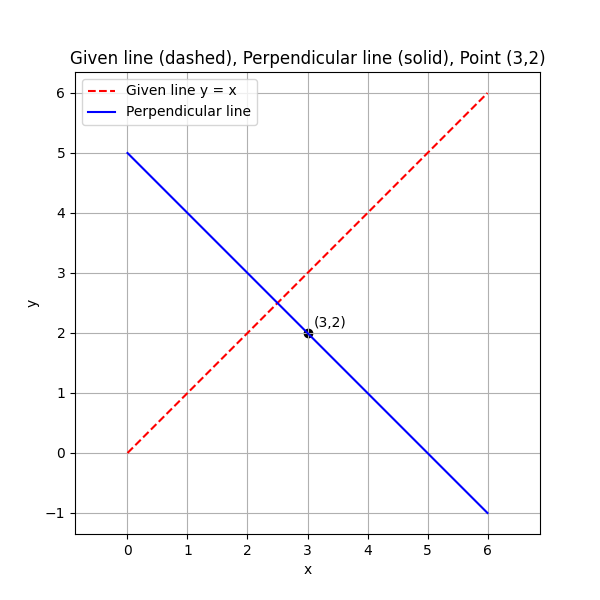
\includegraphics[width=0.5\columnwidth]{figs/2.png}
     \caption{}
     \label{fig:placeholder}
 \end{figure}
\end{frame}
\end{document}

